% Now generating
\documentclass{article}
\usepackage{tikz}
\usetikzlibrary{shapes, arrows, decorations.pathmorphing}
\begin{document}
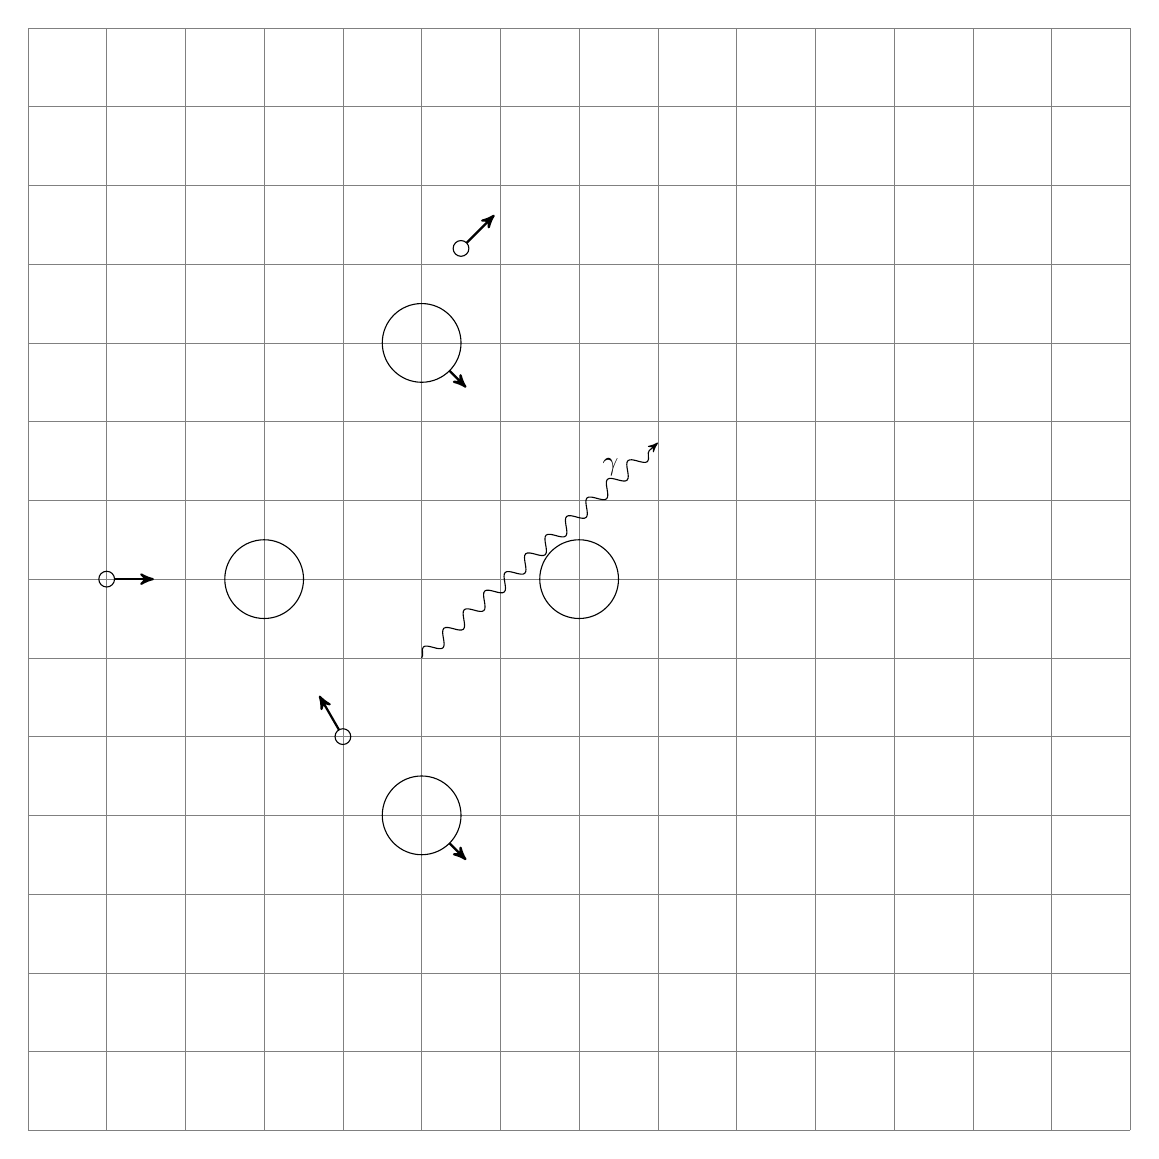
\begin{tikzpicture}[ >=stealth', pos = .8, photon/.style={decorate, decoration = {snake, post length = 1mm}}]
\draw [step = 1cm, gray, very thin] (-7, -7) grid (7,7);
\draw (0,0) circle [radius = 0.5cm];
\draw (-4,0) circle [radius = 0.5cm];
\draw (-6,0) circle [radius = 0.1cm];
\draw [->, thick] (-5.9,0.0) -- (-5.4,0.0);
\draw (-1.5,4.2) circle [radius = 0.1cm];
\draw [->, thick] (-1.42928932188,4.27071067812) -- (-1.07573593129,4.62426406871);
\draw (-2,3) circle [radius = 0.5cm];
\draw [->, thick] (-1.64644660941,2.64644660941) -- (-1.43431457505,2.43431457505);
\draw (-2,-3) circle [radius = 0.5cm];
\draw [->, thick] (-1.64644660941,-3.35355339059) -- (-1.43431457505,-3.56568542495);
\draw (-3,-2) circle [radius = 0.1cm];
\draw [->, thick] (-3.05,-1.91339745962) -- (-3.3,-1.48038475773);
\draw[->, photon] (-2,-1) -- node[above] {$\gamma$} (60:2);\end{tikzpicture}
\end{document}